\chapter{Integración con Google Forms}\label{cap:implementacion-test}
La integración con Google Forms se ha llevado a cabo mediante el desarrollo de plugins que optimizan la recolección y organización de datos a través de formularios. A continuación, se detallan los aspectos clave de esta integración:


\subsubsection{Automatización de la Carga de Preguntas:}
La carga manual de datos para las localidades, provincias y nacionalidades se optimizó mediante una hoja de cálculo con opciones de filtro por nacionalidad y un script generado en Google Apps Script. Estos recursos, están disponibles en el repositorio de la unidad, adicionalmente se deberá establecer vínculos manuales entre preguntas para redirigir a los usuarios a las secciones correspondientes según sus elecciones.

\subsubsection{Manejo de Formularios Específicos:}
Para casos específicos, como el registro de hijos de un consultante, se creó un formulario separado debido a las limitaciones de Google Forms en la gestión dinámica de la cantidad de hijos que un consultante podría tener. Además, se diseñó un formulario exclusivo para consultas, vinculando la consulta con el consultante mediante su documento de identidad (DNI o pasaporte).

\subsubsection{Envío de Datos al Sistema Case Management System:}

Para el envío de la información recopilada a través de los formularios, se implementaron endpoints dedicados para cada tipo de formulario en la API REST. Además, se diseñaron funciones en Google Apps Script que se ejecutan al enviar un formulario, encargadas de recuperar y transformar los datos antes de transmitirlos a la API REST del proyecto. En caso de fallos en este proceso, el sistema notificará a través de correo electrónico sobre la imposibilidad de enviar los datos, asegurando una comunicación eficiente en caso de inconvenientes.

Para obtener información adicional sobre las interfaces, consulte la sección de anexos \ref{cap:anexo-expoint-forms}.


La implementación de estas funcionalidades se puede encontrar en el directorio \href{https://github.com/proyecto-patrocinio/proyecto-patrocinio/tree/main/com/script-forms}{proyecto-patrocinio/com/script-forms/} del repositorio del proyecto. Para incorporar estos archivos al formulario correspondiente, simplemente abra el editor del formulario, seleccione los tres puntos, vaya a "Editor de secuencias de comandos" y agregue los archivos correspondientes.




\begin{figure}[H]
\centering
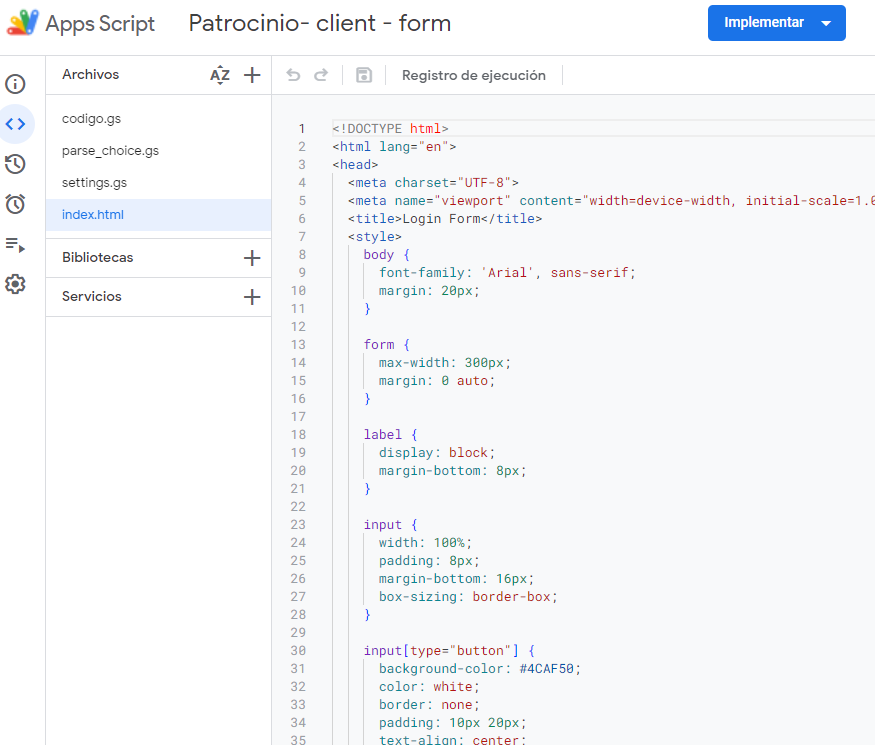
\includegraphics[width=0.75\linewidth]{fig/app-script-code.png}
\caption{Captura de pantalla del código en Google Apps Script.}
\label{fig:app-script-code}
\end{figure}

Adicionalmente, se deben configurar los activadores siguiendo las instrucciones del README del repositorio. Por ejemplo, en el formulario ``Clients'', se necesitan los activadores: ``onFormOpen'' (explicado en la sección \ref{subsubsec:app-script-menu}), ``updateCredentials'' (explicado en la sección \ref{subsubsec:refresh-token}) y ``onFormSubmit''.

\begin{figure}[H]
\centering
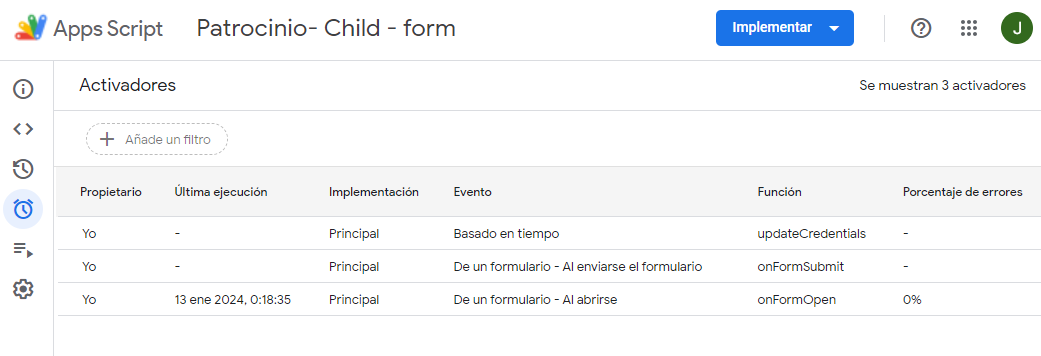
\includegraphics[width=0.90\linewidth]{fig/activadores.png}
\caption{Configuración de activadores.}
\label{fig:activadores}
\end{figure}

El activador ``onFormSubmit'' debe agregarse a los tres formularios y se encargará de ejecutar las funciones para el envío del formulario a la API.

\begin{figure}[H]
\centering
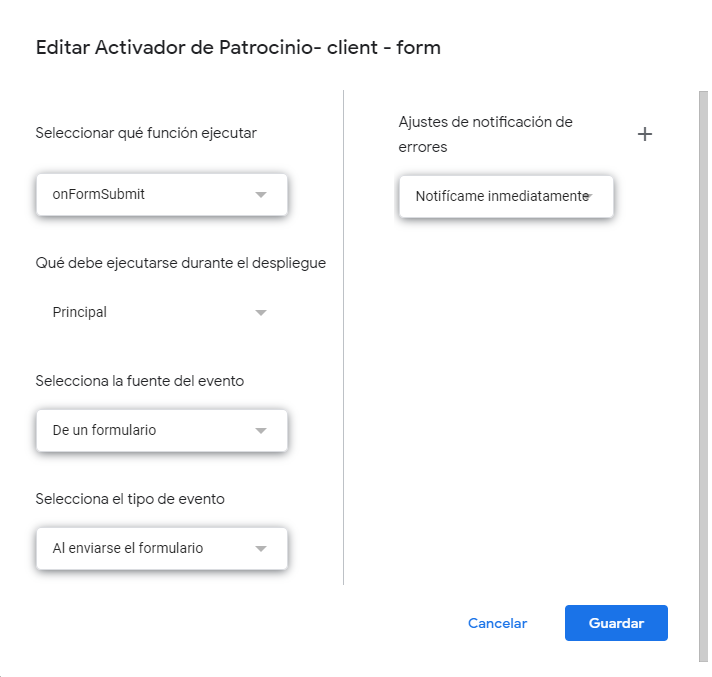
\includegraphics[width=0.75\linewidth]{fig/activador-api-send-form.png}
\caption{Activador para el envío del formulario a la API.}
\label{fig:activador-api-send-form}
\end{figure}





\subsubsection{Seguridad y Autenticación:}\label{subsubsec:app-script-menu}
Se estableció un rol especial para Google Forms con el fin de garantizar la conexión segura con el sistema. Se requiere proporcionar las credenciales de un usuario con este rol en cada formulario. Para facilitar la gestión de estas credenciales, se implementó un plugin de menú mediante Google Apps Script, ofreciendo opciones para cargar credenciales y refrescar tokens de forma intuitiva.

La implementación de esta funcionalidad implica agregar los archivos del directorio \href{https://github.com/proyecto-patrocinio/proyecto-patrocinio/tree/main/com/script-forms/common}{proyecto-patrocinio/com/script-forms/common} del repositorio en los tres formularios.

En la Figura \ref{fig:forms-menu-1}, se muestra la ubicación del plugin del menú en la esquina superior derecha del formulario.

\begin{figure}[H]
    \centering
    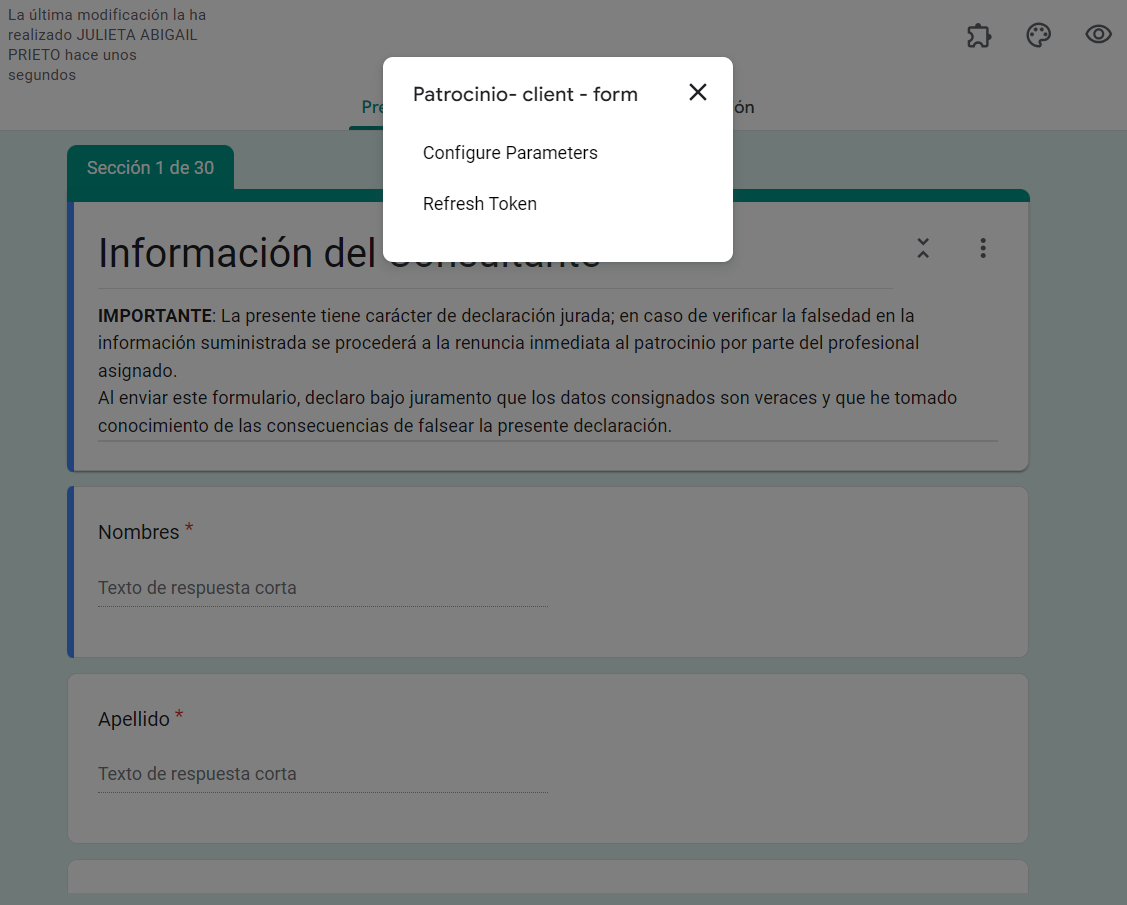
\includegraphics[width=1\linewidth]{fig/forms-menu-2.png}
    \caption{Ubicación del Plugin de Menú en Google Forms}
    \label{fig:forms-menu-1}
\end{figure}

En la Figura \ref{fig:froms-menu-parameters}, se presenta la interfaz de configuración del plugin. Aquí, se debe establecer, por única vez, el nombre de usuario y la contraseña del usuario de Case Managment System con permisos específicos para ``forms'', la URL para iniciar sesión, es decir \textbf{https://\{\{domain\}\}/api/auth/login/}, y la URL del endpoint correspondiente, como por ejemplo \textbf{https://\{\{domain\}\}/api/consultations/consultation/form/} para el formulario de consultantes.

\begin{figure}[H]
    \centering
    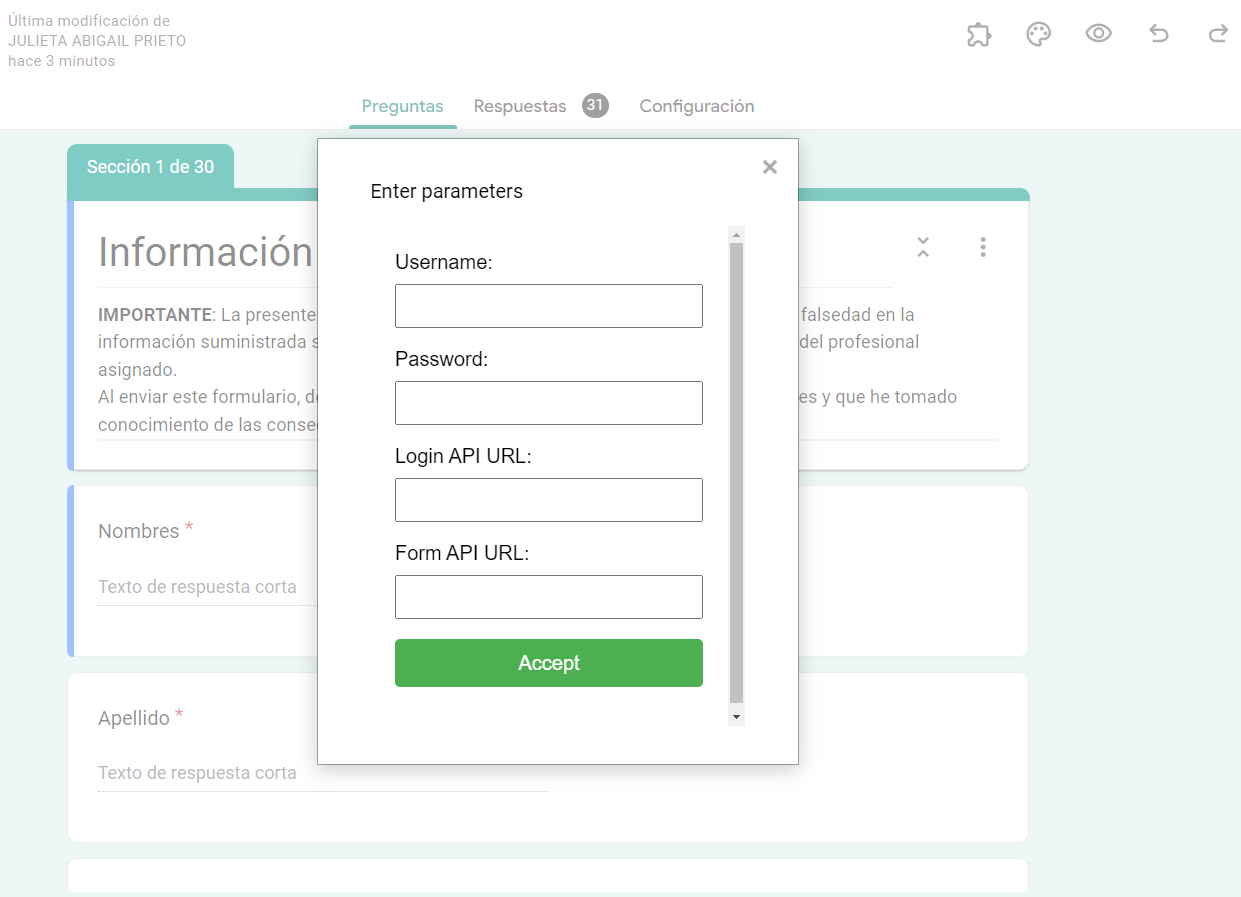
\includegraphics[width=1\linewidth]{fig/forms-menu-parametros.png}
    \caption{Interfaz de Configuración del Plugin de Menú}
    \label{fig:froms-menu-parameters}
\end{figure}

Para obtener información detallada, consulte el README y los archivos de notas en cada directorio correspondiente al formulario en el repositorio.

\subsubsection{Refresco Automático de Tokens:}\label{subsubsec:refresh-token}

Con el objetivo de mejorar la eficiencia del sistema, se ha implementado un activador que ejecuta automáticamente el proceso de refresco del token en intervalos regulares. Aunque es posible realizar este proceso manualmente, se recomienda configurar la opción automática para garantizar la continuidad segura de la conexión.

Para implementar esta funcionalidad, además de agregar los archivos del directorio \href{https://github.com/proyecto-patrocinio/proyecto-patrocinio/tree/main/com/script-forms/common}{proyecto-patrocinio/com/script-forms/common} en el repositorio, es necesario crear manualmente el activador. Se sugiere configurar el activador para que ejecute el refresco del token diariamente, preferiblemente durante un horario nocturno.

En la Figura \ref{fig:activador-credentials-form}, se muestra cómo crear el activador de forma manual.

\begin{figure}[H]
    \centering
    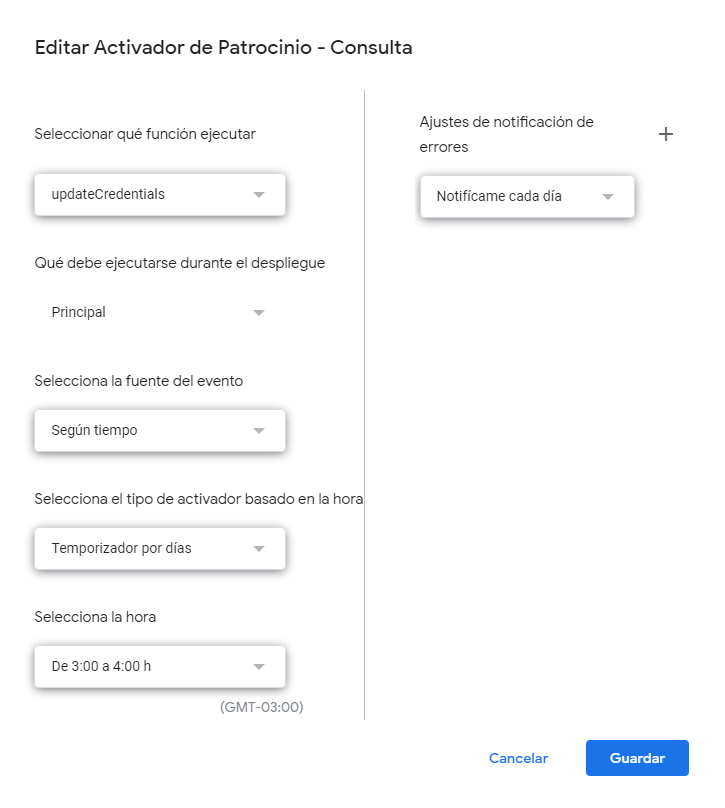
\includegraphics[width=1\linewidth]{fig/activador-credentials-form.png}
    \caption{Activador para el Refresco Automático del Token}
    \label{fig:activador-credentials-form}
\end{figure}

